\documentclass[lang=en,11pt,a4paper]{elegantpaper}

\usepackage{float}
\hypersetup{hidelinks}
\usepackage{tabularx}

% Title
\title{Design of Enterprise IoT: Assignment 1a\\[0.4em]
	\large Smart Turtle Breeding System (STBS)}
	

% Team Members
\author{Team 01}

\institute{Jinling Institute of Technology}
\date{\today}

\begin{document}

\maketitle
\begin{center}
	\renewcommand{\arraystretch}{0.8}
	\begin{tabularx}{0.98\textwidth}{@{}llXX@{}}
		\toprule
		\textbf{Student ID} &
		\textbf{Name} &
		\textbf{Preferred Name} &
		\textbf{Contribution (\%)} \\
		\midrule
		2422441049 & Li Jingru      & Leamon & 25\% \\
		2422441046 & Rong Yicheng   & Bacon  & 25\% \\
		2422441050 & Zhang Zhengyan & Paul   & 25\% \\
		2422441048 & Ye Taohao      & Leaf   & 25\% \\
		\bottomrule
	\end{tabularx}
\end{center}

\section{Task 1: Use Case Description}

A Chinese soft-shell turtle farm operates 20 indoor or semi-closed aquaculture units with an operations and maintenance team. Farm operators manage water quality, feeding, temperature, turtle activity and nesting areas; maintenance technicians service filters and pumps.

Operators manually measure water conditions, prepare feed, inspect behaviour and health, change water, and search for eggs. Periodic rounds can cause inconsistent feeding, delayed detection of deteriorating conditions or equipment failures, and labour-intensive egg collection. Water quality, feeding and temperature affect turtle health and growth~[1]. Reviews identify temperature, dissolved oxygen and pH as priority IoT aquaculture parameters~[2, 3].

An IoT solution is proposed to monitor behavioural conditions continuously, control feeding and temperature, and support bounded partial water changes. Distributed sensors, actuators and cameras send alerts and records so one team can respond between rounds; field evidence shows that vision-based nesting detection can reduce egg-harvesting effort~[4].


\section{Task 2: Solution Overview}

STBS uses water-temperature, pH, turbidity and ammonia sensors in each unit, with level/flow feedback, feeder sensors and IP cameras covering activity, feeding and nesting zones. Local controllers compare readings with species- and growth-stage set-points, regulate heaters, dispense scheduled portions and perform bounded partial water changes. Device feedback and follow-up measurements verify each action. An edge gateway keeps essential rules operating during internet loss, filters routine data and sends readings, events and selected video to a cloud dashboard. Alerts identify the affected unit, abnormal parameter, action taken and need for intervention. Farm operators configure targets, review alerts and nesting evidence, collect eggs and override automation. Maintenance technicians calibrate sensors, service filters and equipment, diagnose failures and maintain power/network availability. Role-based access, audit logs and local fail-safe limits support reliable operation.

\newpage
\section{Task 3: Value Proposition}

The value proposition follows the tutorial method. It distinguishes the current substitute from the proposed system, separates benefits from features, describes the user experience, and records adoption needs and implementation fears. Each statement identifies the stakeholder to whom it applies.

\thispagestyle{plain}
\begin{center}
  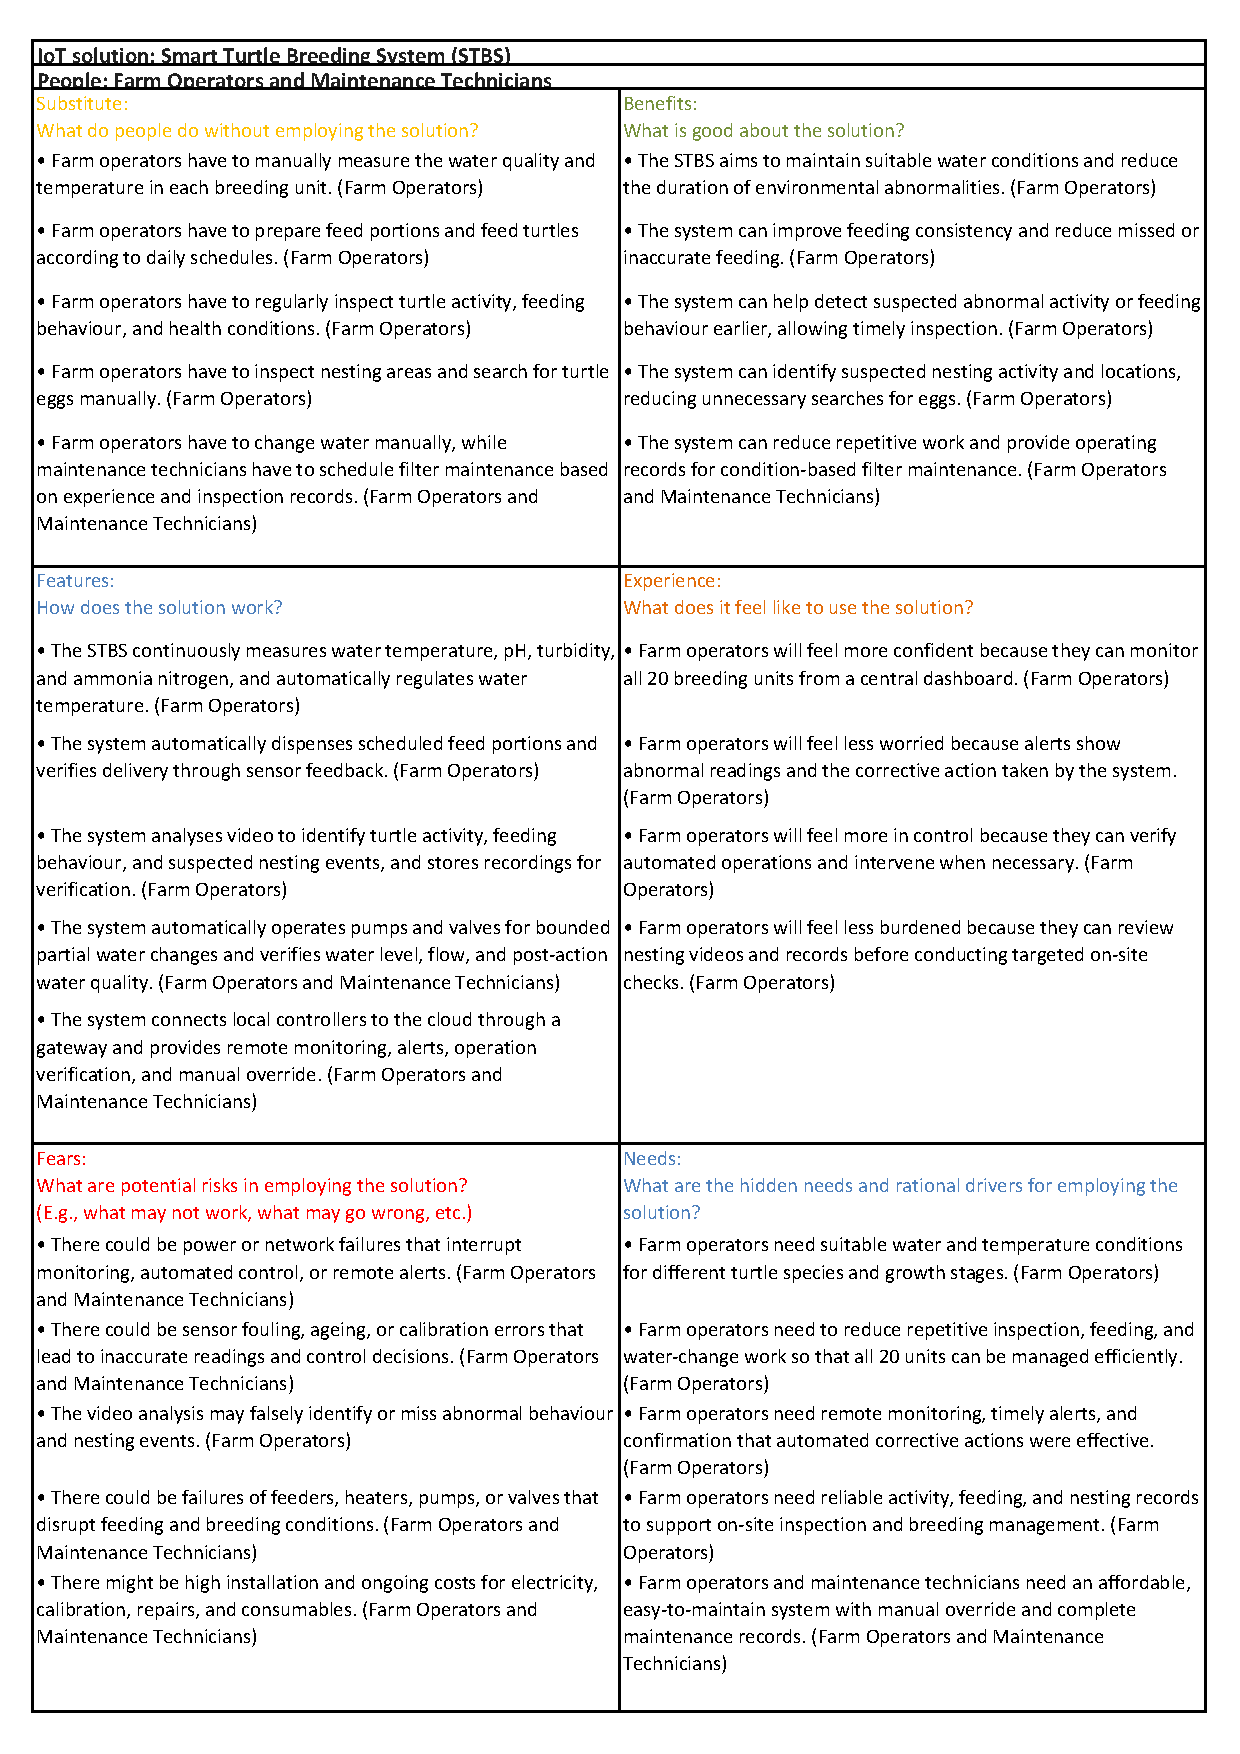
\includegraphics[width=0.95\linewidth,keepaspectratio]{assets/value_proposition_vector.pdf}
\end{center}
\clearpage

\section{References}

\renewcommand{\labelenumi}{[\arabic{enumi}]}
\begin{enumerate}
  \item Food and Agriculture Organization of the United Nations. ``Cultured Aquatic Species Information Programme: Chinese soft-shell turtle (\textit{Trionyx sinensis}).'' Available at \href{https://www.fao.org/fishery/culturedspecies/trionyx_sinensis__en/en}{FAO cultured species profile}.

  \item D. R. Prapti et al. ``Internet of Things (IoT)-based aquaculture: An overview of IoT application on water quality monitoring.'' \textit{Reviews in Aquaculture}, 14, 979--992, 2022. \href{https://doi.org/10.1111/raq.12637}{doi:10.1111/raq.12637}.

  \item H. Rastegari et al. ``Internet of Things in aquaculture: A review of the challenges and potential solutions based on current and future trends.'' \textit{Smart Agricultural Technology}, 4, 100187, 2023. \href{https://doi.org/10.1016/j.atech.2023.100187}{doi:10.1016/j.atech.2023.100187}.

  \item A. Munyaev, B.-L. Jiang, and I.-J. Huang. ``Smart turtle farm: Soft-shell turtle nesting behavior recognition and monitoring system.'' \textit{Computers and Electronics in Agriculture}, 244, 111477, 2026. \href{https://doi.org/10.1016/j.compag.2026.111477}{doi:10.1016/j.compag.2026.111477}.
\end{enumerate}

\end{document}
